\section{从无前缀安全PRF到完全安全PRF(方法1):加密PRF}\label{sec:6-5}

我们下面展示如何将无前缀安全的 PRF $F_{\rm CBC}$ 和 $F^*$ 转换为安全的 PRF,这将为我们提供针对变长输入的安全 MAC。更一般地,我们将展示如何将无前缀安全的 PRF $PF$ 转换为完全安全的 PRF。我们会介绍以下三种方法:
\begin{itemize}
	\item 加密 PRF:用另一个 PRF 对 $PF$ 的短输出进行加密。
	\item 无前缀编码:对 $PF$ 的输入进行编码,使得任意一个输入都不是其他输入的前缀。
	\item CMAC:引入随机化的一种更有效的无前缀编码。
\end{itemize}
在这一节中,我们首先介绍加密 PRF 的方法。这个构造是相当直接的。令 PF 是一个从 $\mathcal{X}^{\leq\ell}$ 映射到 $\mathcal{Y}$ 的 PRF,$F$ 是一个从 $\mathcal{Y}$ 映射到 $\mathcal{T}$ 的 PRF。定义:
\begin{equation}\label{eq:6-17}
EF\big((k_1,k_2),\;m\big)=F\big(k_2,\;PF(k_1,m)\big)
\end{equation}
该构造如图 \ref{fig:6-4} 所示。

\begin{figure}
  \centering
  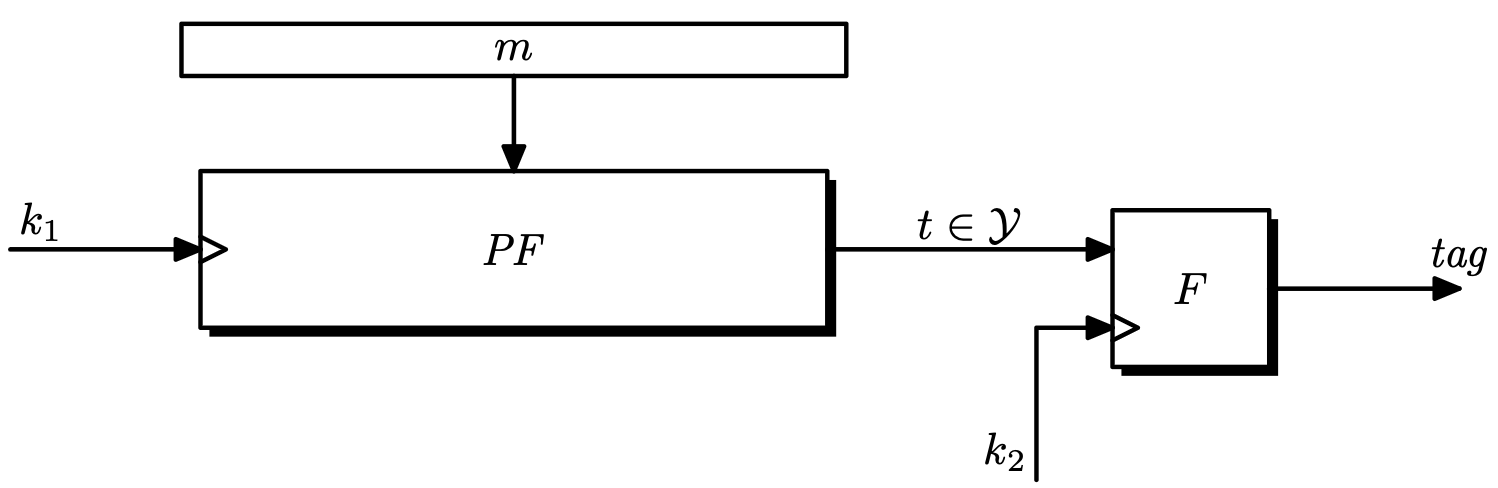
\includegraphics[width=0.65\linewidth]{figures/chapter6/fig4.png}
  \caption{加密 PRF 构造 $EF(k,m)$}
  \label{fig:6-4}
\end{figure}

我们声称,当 $PF$ 是 CBC 或级联中的任何一种构造时,$EF$ 都是一个安全的 PRF。更一般地,我们表明,只要 $PF$ 是一个\emph{可扩展的} PRF,$EF$ 就是安全的。可扩展性的定义如下:

\begin{definition}\label{def:6-4}
令 $PF$ 是一个定义在 $(\mathcal{K},\mathcal{X}^{\leq\ell},\mathcal{Y})$ 上的 PRF。如果对于所有的 $k\in\mathcal{K}$,$x,y\in\mathcal{X}^{\leq\ell-1}$ 和 $a\in\mathcal{X}$,我们都有:
\[
\text{if}\quad
PF(k,x)=PF(k,y)
\quad\text{then}\quad
PF(k,\;x\,\Vert\,a)=PF(k,\;y\,\Vert\,a)
\]
就称 $PF$ 是一个\textbf{可扩展 (extendable) PRF}。
\end{definition}

不难发现,CBC 和级联构造都是可扩展的 PRF。下面的定理将表明,如果 $PF$ 是一个可扩展的无前缀安全 PRF,$EF$ 就是一个安全的 PRF。

\begin{theorem}\label{theo:6-5}
令 $PF$ 是一个定义在 $(\mathcal{K}_1,\mathcal{X}^{\leq\ell+1},\mathcal{Y})$ 上的可扩展且无前缀安全的 PRF,其中 $|\mathcal{Y}|$ 是超多项式的,$\ell$ 是多项式约束的。令 $F$ 是一个定义在 $(\mathcal{K}_2,\mathcal{Y},\mathcal{T})$ 上的安全的 PRF。那么如式 \ref{eq:6-17} 中所定义的 $EF$ 是一个定义在 $(\mathcal{K}_1\times\mathcal{K}_2,\mathcal{X}^{\leq\ell},\mathcal{T})$ 上的安全的 PRF。
\begin{quote}
特别地,对于每个按照攻击游戏 \ref{game:4-2} 攻击 $EF$ 的 PRF 对手 $\mathcal{A}$,假设它最多能够向其挑战者发起 $Q$ 次查询,则必然存在一个按照攻击游戏 \ref{game:4-2} 攻击 $F$ 的 PRF 对手 $\mathcal{B}_1$ 和一个按照攻击游戏 \ref{game:4-2} 攻击 $PF$ 的无前缀 PRF 对手 $\mathcal{B}_2$,其中 $\mathcal{B}_1$ 和 $\mathcal{B}_2$ 都是围绕 $\mathcal{A}$ 的基本包装器,满足:
\end{quote}
\begin{equation}\label{eq:6-18}
{\rm PRF\mathsf{adv}}[\mathcal{A},EF]\leq {\rm PRF\mathsf{adv}}[\mathcal{B}_1,F]+{\rm PRF^{pf}\mathsf{adv}}[\mathcal{B}_2,PF]+\frac{Q^2}{2|\mathcal{Y}|}
\end{equation}
\end{theorem}

\noindent
在我们提供了必要的工具之后,我们将在下一章(\ref{subsec:7-3-1} 小节)证明定理 \ref{theo:6-5}。请注意,为了使 $EF$ 在长度不超过 $\ell$ 的输入上都是安全的 PRF,该定理要求 $PF$ 对于长为 $\ell+1$ 的输入是都无前缀安全的。

\begin{snote}[式 \ref{eq:6-18} 中的上界是严格的。]
虽然不是完全必要,但让我们假设 $\mathcal{Y}=\mathcal{T}$,$F$ 是一个分组密码,并且 $|\mathcal{X}|$ 不是非常小。这些假设将大大简化论证。我们下面展示一种攻击,它能在 $Q\approx\sqrt{|\mathcal{Y}|}$ 次查询之后以恒定概率攻破 $EF$。事实上,我们的攻击将攻破作为一个 MAC 的 $EF$。对手首先挑选 $Q$ 个随机输入 $x_1,\dots,x_Q\in\mathcal{X}^2$,并用这 $Q$ 个输入向其挑战者发起查询,以得到应答 $t_1,\dots,t_Q\in\mathcal{T}$。根据生日悖论(推论 \ref{cor:B-2}),对于任何固定的密钥 $k_1$,存在不同的索引 $i$ 和 $j$ 使得 $x_i\neq x_j$ 且 $PF(k_1,x_i)=PF(k_1,x_j)$ 的概率是恒定的。一方面,如果发生这样的碰撞,我们可以有效发现它,这是因为对于这样的一对索引,必有 $t_i=t_j$。另一方面,如果存在一对索引 $i$ 和 $j$ 使得 $t_i=t_j$,由于我们假设 $F$ 是一个分组密码,那么必然有 $PF(k_1,x_i)=PF(k_1,x_j)$。现在,假设 $x_i\neq x_j$ 且 $PF(k_1,x_i)=PF(k_1,x_j)$,由于 $PF$ 是可扩展的,那么对于任意 $a\in\mathcal{X}$,我们都有 $PF\big(k_1,\,(x_i\,\Vert\,a)\big)=PF\big(k_1,\,(x_j\,\Vert\,a)\big)$。因此,我们的对手可以获得 $x_i\,\Vert\,a$ 的 MAC 标签 $t$,而这个标签 $t$ 同时也是 $x_j\,\Vert\,a$ 的有效标签。推广这一攻击,我们就能很容易地证明式 \ref{eq:6-18} 中 ${Q^2}/{(2|\mathcal{Y}|)}$ 这一项的必要性。
\end{snote}

\subsection{ECBC 和 NMAC:用于变长输入的安全 PRF}

图 \ref{fig:6-5-a} 和 \ref{fig:6-5-b} 展示了对 CBC 和级联应用 $EF$ 构造的结果。

\begin{figure}
  \centering
  \subfigure[ECBC 构造 $\mathrm{ECBC}(k,m)$(加密CBC)]{
  	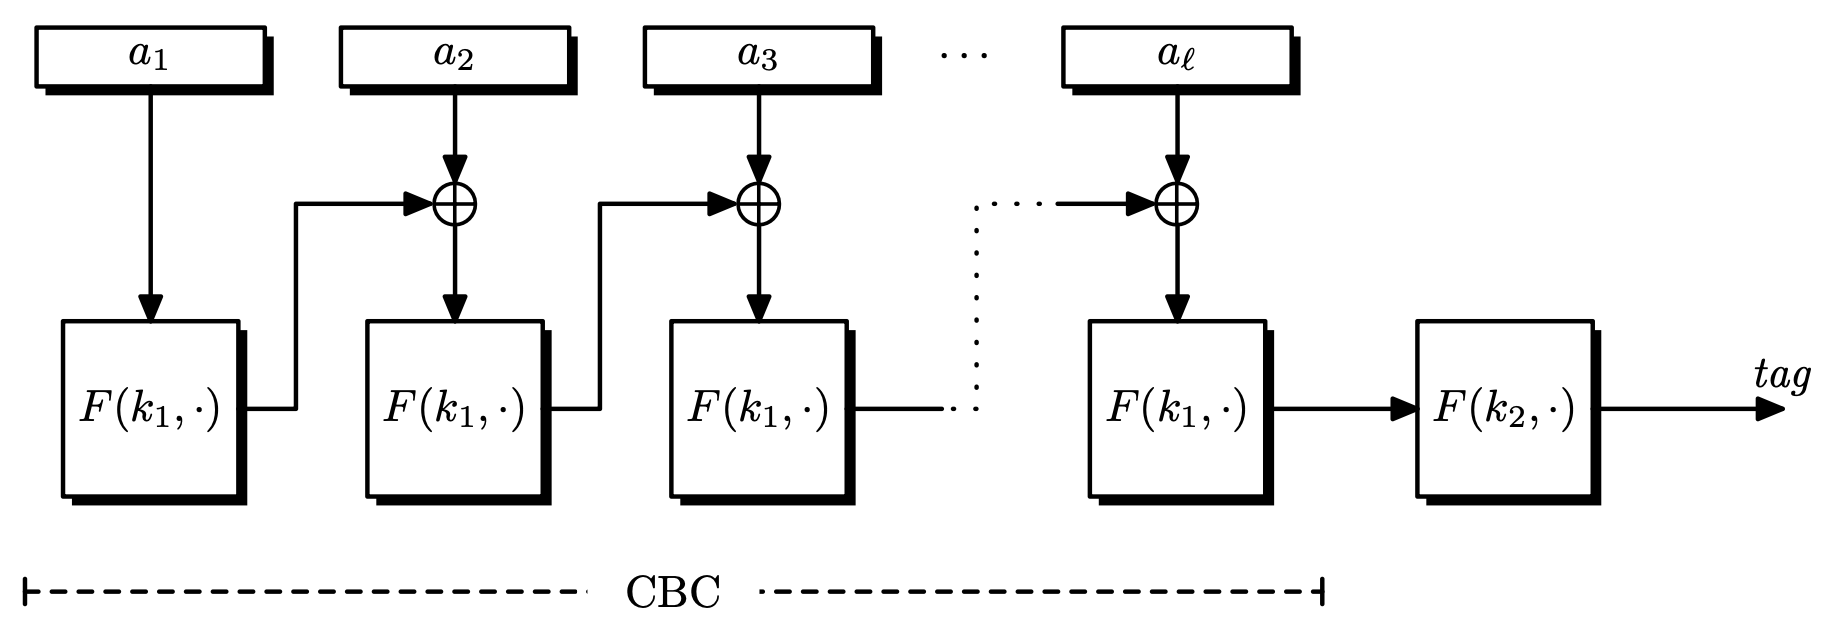
\includegraphics[width=0.8\linewidth]{figures/chapter6/fig5-a.png}
  	\label{fig:6-5-a}
  }
  
  \subfigure[NMAC 构造 $\mathrm{NMAC}(k,m)$(加密级联)]{
  	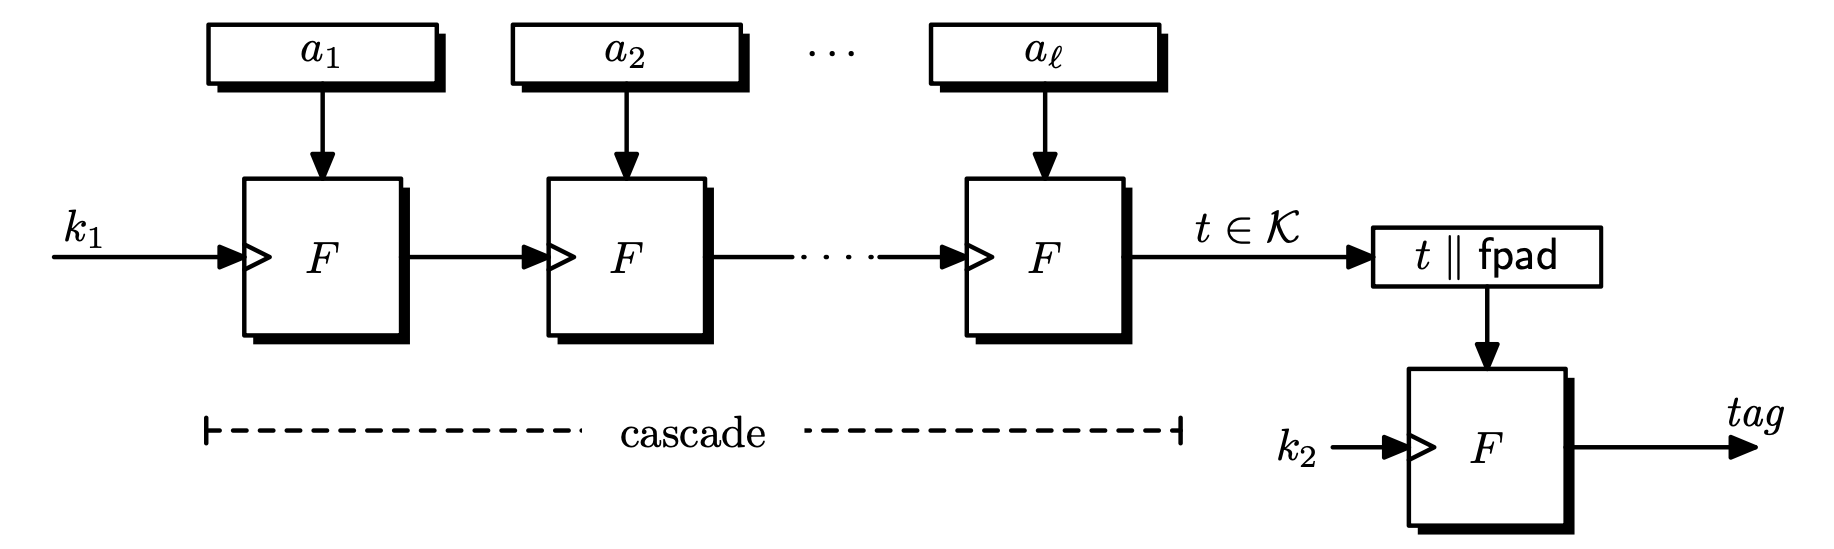
\includegraphics[width=0.8\linewidth]{figures/chapter6/fig5-b.png}
  	\label{fig:6-5-b}
  }
  \caption{用于变长输入的安全 PRF}
\end{figure}

\subsubsection{加密 CBC PRF}

将 $EF$ 应用于 CBC 构造就能得到一个经典的 PRF(因而也是一个 MAC),称为\textbf{加密 CBC (encrypted-CBC)} 或 \textbf{ECBC}。这种 MAC 由 ANSI 标准化(见 \ref{sec:6-9} 节),并被广泛用于银行业。ECBC PRF 在 CBC 和最终的加密中使用相同的底层 PRF $F$。因此,ECBC 定义在 $(\mathcal{K}^2,\mathcal{X}^{\leq\ell+1},\mathcal{X})$ 上。

\begin{theorem}[ECBC 的安全性]\label{theo:6-6}
令 $F$ 是一个定义在 $(\mathcal{K},\mathcal{X},\mathcal{X})$ 上的安全 PRF。假设 $\mathcal{X}$ 是超多项式的,$\ell$ 是一个多项式约束的长度参数。那么 ECBC 是一个定义在 $(\mathcal{K}^2,\mathcal{X}^{\leq\ell+1},\mathcal{X})$ 上的安全 PRF。
\begin{quote}
特别地,对于每个按照攻击游戏 \ref{game:4-2} 攻击 ECBC 的 PRF 对手 $\mathcal{A}$,假设它最多能够向其挑战者发起 $Q$ 次查询,则必然存在两个按照攻击游戏 \ref{game:4-2} 攻击 $F$ 的 PRF 对手 $\mathcal{B}_1$ 和 $\mathcal{B}_2$,其中 $\mathcal{B}_1$ 和 $\mathcal{B}_2$ 都是围绕 $\mathcal{A}$ 的基本包装器,满足:
\end{quote}
\begin{equation}\label{eq:6-19}
{\rm PRF}\mathsf{adv}[\mathcal{A},{\rm ECBC}]\leq{\rm PRF}\mathsf{adv}[\mathcal{B}_1,F]+{\rm PRF}\mathsf{adv}[\mathcal{B}_2,F]+\frac{(Q(l+1))^2+Q^2}{2|\mathcal{X}|}
\end{equation}
\end{theorem}

\begin{proof}
根据定理 \ref{theo:6-3},CBC 显然是可扩展的,而且是一个无前缀安全的 PRF。因此,如果底层 PRF $F$ 是安全的,那么根据定理 \ref{theo:6-5},ECBC 也是一个安全的 PRF。
\end{proof}

定理 \ref{theo:6-5} 之后的论证表明,存在一个攻击者,在 $Q\approx\sqrt{|\mathcal{X}|}$ 次查询后,能以恒定优势破解该 PRF。回顾一下,对于 3DES,我们有 $\mathcal{X}=\{0,1\}^{64}$。因此,在大约 10 亿次(或者更准确地说, $2^{32}$ 次)查询之后,攻击者就能以恒定的概率破解 ECBC-3DES MAC。

\subsubsection{NMAC PRF}

将 $EF$ 应用于级联构造同样能得到一个 PRF(因而也是一个 MAC),称为\textbf{嵌套 MAC (Nested MAC)} 或 \textbf{NMAC}。这种 MAC 的一个变体由 IETF 标准化(见 \ref{subsec:8-7-2} 小节),并被广泛用于互联网协议中。

我们希望使用相同的底层 PRF $F$ 来构造级联和进行最终的加密。但不幸的是,级联的输出在 $\mathcal{K}$ 上,而 $F$ 的输入在 $\mathcal{X}$ 上。为了解决这个问题,我们需要将级联的输出嵌入到 $\mathcal{X}$ 中。更确切地说,我们假设 $|\mathcal{K}|\leq|\mathcal{X}|$,并且有一个可有效计算的双射 $g$,它能将 $\mathcal{K}$ 中的元素映射到 $\mathcal{X}$ 上。比如说,假设 $\mathcal{K}:=\{0,1\}^\kappa$,$\mathcal{X}:=\{0,1\}^n$,其中 $\kappa\leq n$。我们定义 $g(t):=t\,\Vert\,\mathsf{fpad}$,其中 $\mathsf{fpad}$ 是一串 $n-\kappa$ 比特的固定填充序列。这个 $\mathsf{fpad}$ 可以像一串 $0$ 一样简单。通过这种转换,所有的 NMAC 都可以由一个安全的 PRF $F$ 构造出来,就如图 \ref{fig:6-5-b} 所示。

\begin{theorem}[NMAC 的安全性]\label{theo:6-7}
令 $F$ 是一个定义在 $(\mathcal{K},\mathcal{X},\mathcal{K})$ 上的安全的 PRF,其中 $\mathcal{K}$ 可以嵌入到 $\mathcal{X}$ 中,那么 NMAC 就是一个定义在 $(\mathcal{K}^2,\mathcal{X}^{\leq\ell},\mathcal{K})$ 上的安全的 PRF。
\begin{quote}
特别地,对于每个按照攻击游戏 \ref{game:4-2} 攻击 NMAC 的 PRF 对手 $\mathcal{A}$,假设它最多能够向其挑战者发起 $Q$ 次查询,则必然存在两个按照攻击游戏 \ref{game:4-2} 攻击 $F$ 的 PRF 对手 $\mathcal{B}_1$ 和 $\mathcal{B}_2$,其中 $\mathcal{B}_1$ 和 $\mathcal{B}_2$ 都是围绕 $\mathcal{A}$ 的基本包装器,满足:
\end{quote}
\begin{equation}\label{eq:6-20}
{\rm PRF}\mathsf{adv}[\mathcal{A},{\rm NMAC}]\leq (Q(\ell+1))\cdot{\rm PRF}\mathsf{adv}[\mathcal{B}_1,F]+{\rm PRF}\mathsf{adv}[\mathcal{B}_2,F]+\frac{Q^2}{2|\mathcal{K}|}
\end{equation}
\end{theorem}

\begin{proof}
根据定理 \ref{theo:6-4},NMAC 显然是可扩展的,而且是一个无前缀安全的 PRF。因此,如果底层 PRF $F$ 是安全的,那么根据定理 \ref{theo:6-5},NMAC 也是一个安全的 PRF。
\end{proof}

\begin{snote}[ECBC 和 NMAC 都是流式 MAC。]
ECBC 和 NMAC 都可以用来认证 $\mathcal{X}^{\leq l}$ 上的变长消息。此外,我们并不需要提前知晓消息的长度。具有这种特性的 MAC 被称为\textbf{流式 MAC (streaming MAC)}。这一特性使得应用程序能够一次向 MAC 提供一个消息分组,并在任意位置决定消息是否结束。这对于像流媒体视频这样的应用很重要,因为在这种应用中,应用程序也无法预知消息的长度。

相比之下,一些 MAC 系统要求将消息长度预加到消息正文中(见 \ref{sec:6-6} 节)。这样的 MAC 在实践中更难使用,因为它们要求应用程序在开始计算 MAC 之前就确定消息的长度。
\end{snote}